\documentclass[1p]{elsarticle_modified}
%\bibliographystyle{elsarticle-num}

%\usepackage[colorlinks]{hyperref}
%\usepackage{abbrmath_seonhwa} %\Abb, \Ascr, \Acal ,\Abf, \Afrak
\usepackage{amsfonts}
\usepackage{amssymb}
\usepackage{amsmath}
\usepackage{amsthm}
\usepackage{scalefnt}
\usepackage{amsbsy}
\usepackage{kotex}
\usepackage{caption}
\usepackage{subfig}
\usepackage{color}
\usepackage{graphicx}
\usepackage{xcolor} %% white, black, red, green, blue, cyan, magenta, yellow
\usepackage{float}
\usepackage{setspace}
\usepackage{hyperref}

\usepackage{tikz}
\usetikzlibrary{arrows}

\usepackage{multirow}
\usepackage{array} % fixed length table
\usepackage{hhline}

%%%%%%%%%%%%%%%%%%%%%
\makeatletter
\renewcommand*\env@matrix[1][\arraystretch]{%
	\edef\arraystretch{#1}%
	\hskip -\arraycolsep
	\let\@ifnextchar\new@ifnextchar
	\array{*\c@MaxMatrixCols c}}
\makeatother %https://tex.stackexchange.com/questions/14071/how-can-i-increase-the-line-spacing-in-a-matrix
%%%%%%%%%%%%%%%

\usepackage[normalem]{ulem}

\newcommand{\msout}[1]{\ifmmode\text{\sout{\ensuremath{#1}}}\else\sout{#1}\fi}
%SOURCE: \msout is \stkout macro in https://tex.stackexchange.com/questions/20609/strikeout-in-math-mode

\newcommand{\cancel}[1]{
	\ifmmode
	{\color{red}\msout{#1}}
	\else
	{\color{red}\sout{#1}}
	\fi
}

\newcommand{\add}[1]{
	{\color{blue}\uwave{#1}}
}

\newcommand{\replace}[2]{
	\ifmmode
	{\color{red}\msout{#1}}{\color{blue}\uwave{#2}}
	\else
	{\color{red}\sout{#1}}{\color{blue}\uwave{#2}}
	\fi
}

\newcommand{\Sol}{\mathcal{S}} %segment
\newcommand{\D}{D} %diagram
\newcommand{\A}{\mathcal{A}} %arc


%%%%%%%%%%%%%%%%%%%%%%%%%%%%%5 test

\def\sl{\operatorname{\textup{SL}}(2,\Cbb)}
\def\psl{\operatorname{\textup{PSL}}(2,\Cbb)}
\def\quan{\mkern 1mu \triangleright \mkern 1mu}

\theoremstyle{definition}
\newtheorem{thm}{Theorem}[section]
\newtheorem{prop}[thm]{Proposition}
\newtheorem{lem}[thm]{Lemma}
\newtheorem{ques}[thm]{Question}
\newtheorem{cor}[thm]{Corollary}
\newtheorem{defn}[thm]{Definition}
\newtheorem{exam}[thm]{Example}
\newtheorem{rmk}[thm]{Remark}
\newtheorem{alg}[thm]{Algorithm}

\newcommand{\I}{\sqrt{-1}}
\begin{document}

%\begin{frontmatter}
%
%\title{Boundary parabolic representations of knots up to 8 crossings}
%
%%% Group authors per affiliation:
%\author{Yunhi Cho} 
%\address{Department of Mathematics, University of Seoul, Seoul, Korea}
%\ead{yhcho@uos.ac.kr}
%
%
%\author{Seonhwa Kim} %\fnref{s_kim}}
%\address{Center for Geometry and Physics, Institute for Basic Science, Pohang, 37673, Korea}
%\ead{ryeona17@ibs.re.kr}
%
%\author{Hyuk Kim}
%\address{Department of Mathematical Sciences, Seoul National University, Seoul 08826, Korea}
%\ead{hyukkim@snu.ac.kr}
%
%\author{Seokbeom Yoon}
%\address{Department of Mathematical Sciences, Seoul National University, Seoul, 08826,  Korea}
%\ead{sbyoon15@snu.ac.kr}
%
%\begin{abstract}
%We find all boundary parabolic representation of knots up to 8 crossings.
%
%\end{abstract}
%\begin{keyword}
%    \MSC[2010] 57M25 
%\end{keyword}
%
%\end{frontmatter}

%\linenumbers
%\tableofcontents
%
\newcommand\colored[1]{\textcolor{white}{\rule[-0.35ex]{0.8em}{1.4ex}}\kern-0.8em\color{red} #1}%
%\newcommand\colored[1]{\textcolor{white}{ #1}\kern-2.17ex	\textcolor{white}{ #1}\kern-1.81ex	\textcolor{white}{ #1}\kern-2.15ex\color{red}#1	}

{\Large $\underline{11a_{208}~(K11a_{208})}$}

\setlength{\tabcolsep}{10pt}
\renewcommand{\arraystretch}{1.6}
\vspace{1cm}\begin{tabular}{m{100pt}>{\centering\arraybackslash}m{274pt}}
\multirow{5}{120pt}{
	\centering
	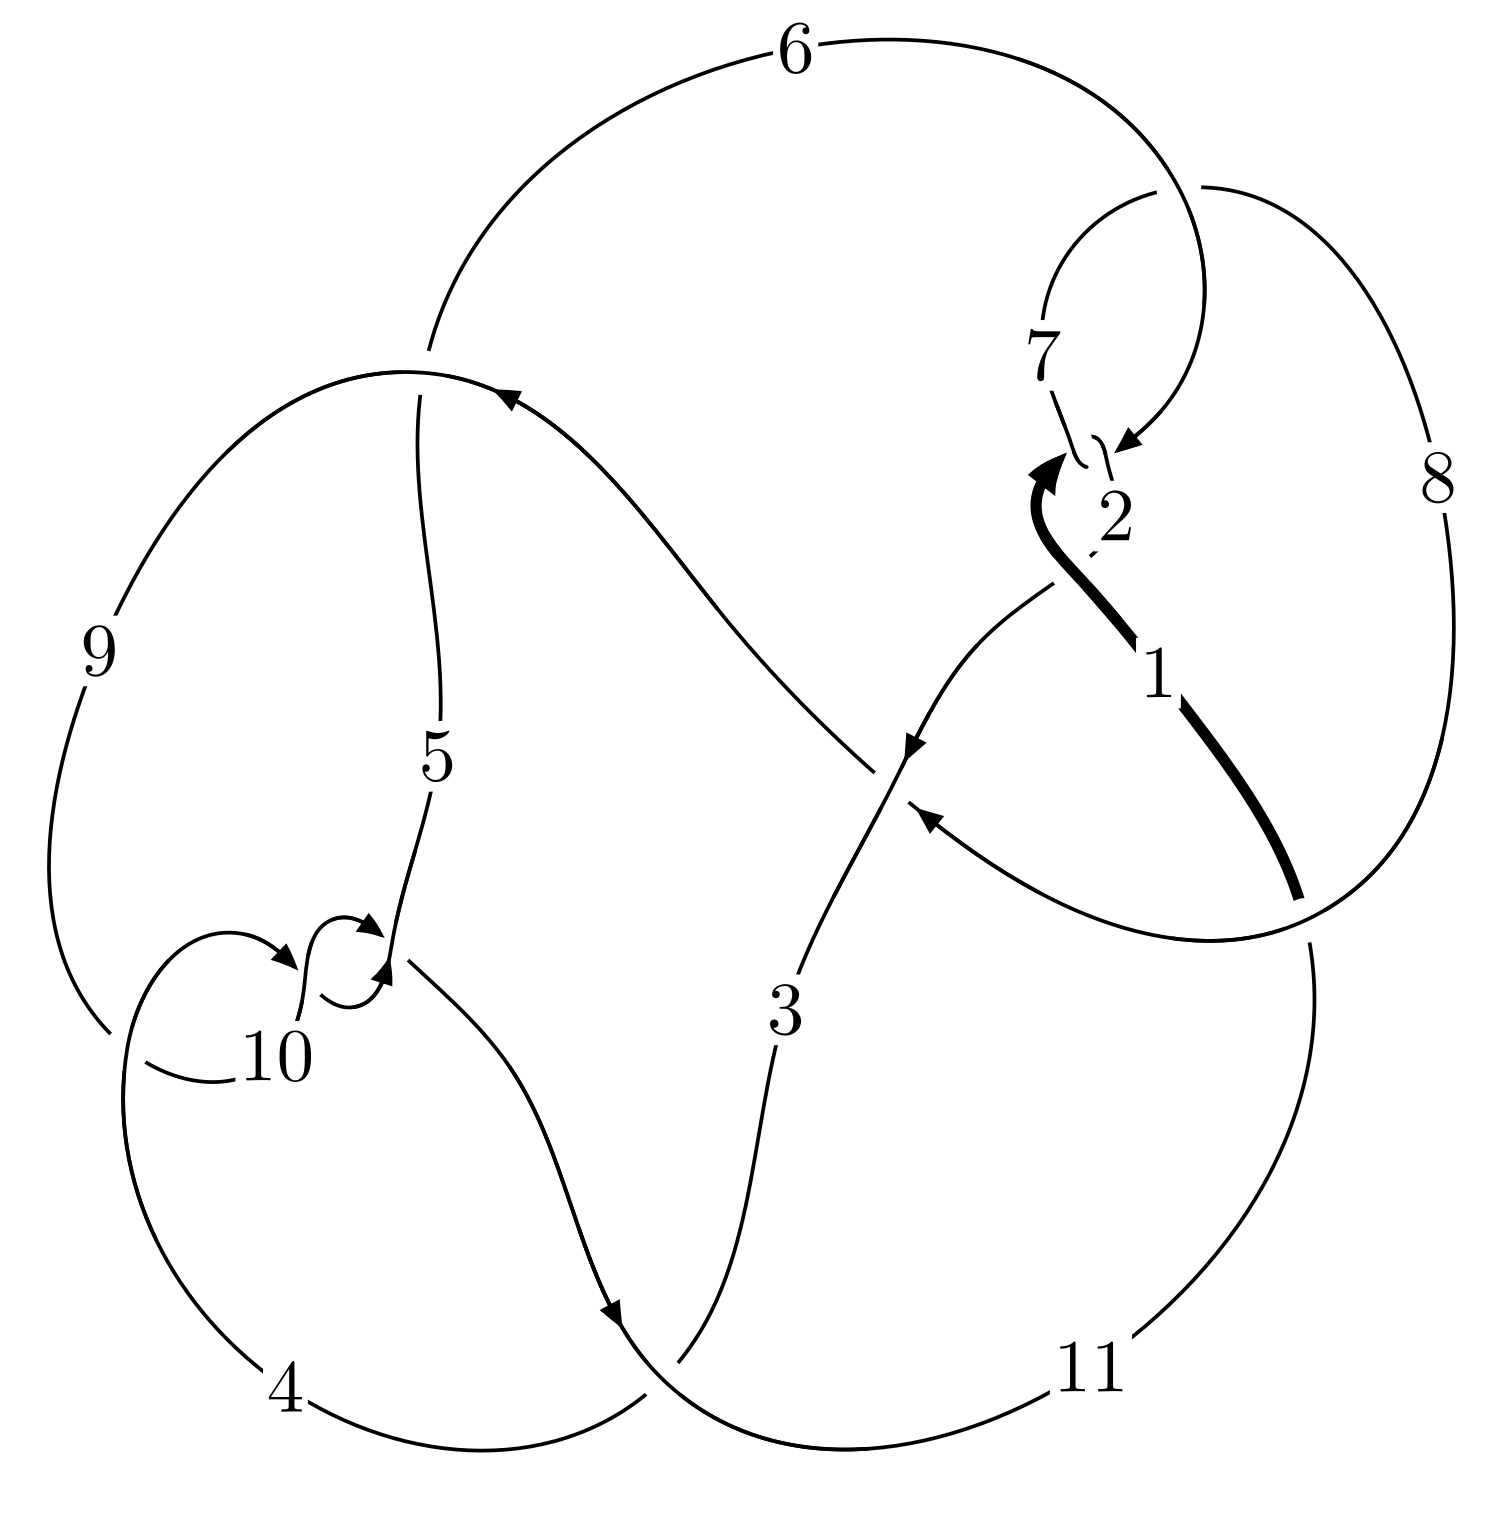
\includegraphics[width=112pt]{../../../GIT/diagram.site/Diagrams/png/457_11a_208.png}\\
\ \ \ A knot diagram\footnotemark}&
\allowdisplaybreaks
\textbf{Linearized knot diagam} \\
\cline{2-2}
 &
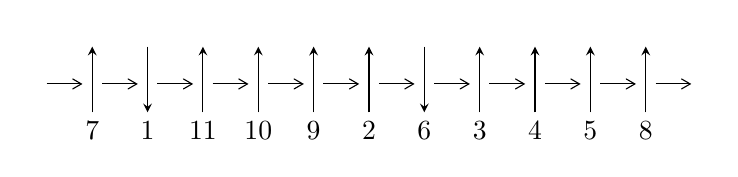
\begin{tikzpicture}[x=20pt, y=17pt]
	% nodes
	\node (C0) at (0, 0) {};
	\node (C1) at (1, 0) {};
	\node (C1U) at (1, +1) {};
	\node (C1D) at (1, -1) {7};

	\node (C2) at (2, 0) {};
	\node (C2U) at (2, +1) {};
	\node (C2D) at (2, -1) {1};

	\node (C3) at (3, 0) {};
	\node (C3U) at (3, +1) {};
	\node (C3D) at (3, -1) {11};

	\node (C4) at (4, 0) {};
	\node (C4U) at (4, +1) {};
	\node (C4D) at (4, -1) {10};

	\node (C5) at (5, 0) {};
	\node (C5U) at (5, +1) {};
	\node (C5D) at (5, -1) {9};

	\node (C6) at (6, 0) {};
	\node (C6U) at (6, +1) {};
	\node (C6D) at (6, -1) {2};

	\node (C7) at (7, 0) {};
	\node (C7U) at (7, +1) {};
	\node (C7D) at (7, -1) {6};

	\node (C8) at (8, 0) {};
	\node (C8U) at (8, +1) {};
	\node (C8D) at (8, -1) {3};

	\node (C9) at (9, 0) {};
	\node (C9U) at (9, +1) {};
	\node (C9D) at (9, -1) {4};

	\node (C10) at (10, 0) {};
	\node (C10U) at (10, +1) {};
	\node (C10D) at (10, -1) {5};

	\node (C11) at (11, 0) {};
	\node (C11U) at (11, +1) {};
	\node (C11D) at (11, -1) {8};
	\node (C12) at (12, 0) {};

	% arrows
	\draw[->,>={angle 60}]
	(C0) edge (C1) (C1) edge (C2) (C2) edge (C3) (C3) edge (C4) (C4) edge (C5) (C5) edge (C6) (C6) edge (C7) (C7) edge (C8) (C8) edge (C9) (C9) edge (C10) (C10) edge (C11) (C11) edge (C12) ;	\draw[->,>=stealth]
	(C1D) edge (C1U) (C2U) edge (C2D) (C3D) edge (C3U) (C4D) edge (C4U) (C5D) edge (C5U) (C6D) edge (C6U) (C7U) edge (C7D) (C8D) edge (C8U) (C9D) edge (C9U) (C10D) edge (C10U) (C11D) edge (C11U) ;
	\end{tikzpicture} \\
\hhline{~~} \\& 
\textbf{Solving Sequence} \\ \cline{2-2} 
 &
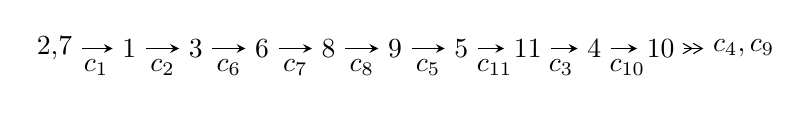
\begin{tikzpicture}[x=24pt, y=7pt]
	% node
	\node (A0) at (-1/8, 0) {2,7};
	\node (A1) at (1, 0) {1};
	\node (A2) at (2, 0) {3};
	\node (A3) at (3, 0) {6};
	\node (A4) at (4, 0) {8};
	\node (A5) at (5, 0) {9};
	\node (A6) at (6, 0) {5};
	\node (A7) at (7, 0) {11};
	\node (A8) at (8, 0) {4};
	\node (A9) at (9, 0) {10};
	\node (C1) at (1/2, -1) {$c_{1}$};
	\node (C2) at (3/2, -1) {$c_{2}$};
	\node (C3) at (5/2, -1) {$c_{6}$};
	\node (C4) at (7/2, -1) {$c_{7}$};
	\node (C5) at (9/2, -1) {$c_{8}$};
	\node (C6) at (11/2, -1) {$c_{5}$};
	\node (C7) at (13/2, -1) {$c_{11}$};
	\node (C8) at (15/2, -1) {$c_{3}$};
	\node (C9) at (17/2, -1) {$c_{10}$};
	\node (A10) at (41/4, 0) {$c_{4},c_{9}$};

	% edge
	\draw[->,>=stealth]	
	(A0) edge (A1) (A1) edge (A2) (A2) edge (A3) (A3) edge (A4) (A4) edge (A5) (A5) edge (A6) (A6) edge (A7) (A7) edge (A8) (A8) edge (A9) ;
	\draw[->>,>={angle 60}]	
	(A9) edge (A10);
\end{tikzpicture} \\ 

\end{tabular} \\

\footnotetext{
The image of knot diagram is generated by the software ``\textbf{Draw programme}" developed by Andrew Bartholomew(\url{http://www.layer8.co.uk/maths/draw/index.htm\#Running-draw}), where we modified some parts for our purpose(\url{https://github.com/CATsTAILs/LinksPainter}).
}\phantom \\ \newline 
\centering \textbf{Ideals for irreducible components\footnotemark of $X_{\text{par}}$} 
 
\begin{align*}
I^u_{1}&=\langle 
u^{52}+u^{51}+\cdots+2 u-1\rangle \\
\\
\end{align*}
\raggedright * 1 irreducible components of $\dim_{\mathbb{C}}=0$, with total 52 representations.\\
\footnotetext{All coefficients of polynomials are rational numbers. But the coefficients are sometimes approximated in decimal forms when there is not enough margin.}
\newpage
\renewcommand{\arraystretch}{1}
\centering \section*{I. $I^u_{1}= \langle u^{52}+u^{51}+\cdots+2 u-1 \rangle$}
\flushleft \textbf{(i) Arc colorings}\\
\begin{tabular}{m{7pt} m{180pt} m{7pt} m{180pt} }
\flushright $a_{2}=$&$\begin{pmatrix}1\\0\end{pmatrix}$ \\
\flushright $a_{7}=$&$\begin{pmatrix}0\\u\end{pmatrix}$ \\
\flushright $a_{1}=$&$\begin{pmatrix}1\\u^2\end{pmatrix}$ \\
\flushright $a_{3}=$&$\begin{pmatrix}u^2+1\\u^4\end{pmatrix}$ \\
\flushright $a_{6}=$&$\begin{pmatrix}- u\\u\end{pmatrix}$ \\
\flushright $a_{8}=$&$\begin{pmatrix}- u^3\\u^3+u\end{pmatrix}$ \\
\flushright $a_{9}=$&$\begin{pmatrix}u^9+2 u^7+3 u^5+2 u^3+u\\u^{11}+u^9+2 u^7+u^5+u^3+u\end{pmatrix}$ \\
\flushright $a_{5}=$&$\begin{pmatrix}- u^{21}-4 u^{19}+\cdots-2 u^3- u\\- u^{23}-3 u^{21}+\cdots-2 u^3+u\end{pmatrix}$ \\
\flushright $a_{11}=$&$\begin{pmatrix}- u^8- u^6- u^4+1\\u^8+2 u^6+2 u^4+2 u^2\end{pmatrix}$ \\
\flushright $a_{4}=$&$\begin{pmatrix}u^{20}+3 u^{18}+7 u^{16}+10 u^{14}+10 u^{12}+7 u^{10}+u^8-2 u^6-3 u^4- u^2+1\\- u^{20}-4 u^{18}-10 u^{16}-18 u^{14}-23 u^{12}-24 u^{10}-18 u^8-10 u^6-3 u^4\end{pmatrix}$ \\
\flushright $a_{10}=$&$\begin{pmatrix}u^{51}+8 u^{49}+\cdots+u^3+2 u\\- u^{51}-9 u^{49}+\cdots+u^3+u\end{pmatrix}$\\ \flushright $a_{10}=$&$\begin{pmatrix}u^{51}+8 u^{49}+\cdots+u^3+2 u\\- u^{51}-9 u^{49}+\cdots+u^3+u\end{pmatrix}$\\&\end{tabular}
\flushleft \textbf{(ii) Obstruction class $= -1$}\\~\\
\flushleft \textbf{(iii) Cusp Shapes $= 4 u^{50}+4 u^{49}+\cdots+4 u^2+14$}\\~\\
\newpage\renewcommand{\arraystretch}{1}
\flushleft \textbf{(iv) u-Polynomials at the component}\newline \\
\begin{tabular}{m{50pt}|m{274pt}}
Crossings & \hspace{64pt}u-Polynomials at each crossing \\
\hline $$\begin{aligned}c_{1},c_{6}\end{aligned}$$&$\begin{aligned}
&u^{52}+u^{51}+\cdots+2 u-1
\end{aligned}$\\
\hline $$\begin{aligned}c_{2},c_{7}\end{aligned}$$&$\begin{aligned}
&u^{52}+17 u^{51}+\cdots-6 u+1
\end{aligned}$\\
\hline $$\begin{aligned}c_{3},c_{5}\end{aligned}$$&$\begin{aligned}
&u^{52}+3 u^{51}+\cdots+37 u+16
\end{aligned}$\\
\hline $$\begin{aligned}c_{4},c_{9},c_{10}\end{aligned}$$&$\begin{aligned}
&u^{52}- u^{51}+\cdots+3 u^2-1
\end{aligned}$\\
\hline $$\begin{aligned}c_{8}\end{aligned}$$&$\begin{aligned}
&u^{52}+u^{51}+\cdots-28 u-40
\end{aligned}$\\
\hline $$\begin{aligned}c_{11}\end{aligned}$$&$\begin{aligned}
&u^{52}-5 u^{51}+\cdots+96 u-16
\end{aligned}$\\
\hline
\end{tabular}\\~\\
\newpage\renewcommand{\arraystretch}{1}
\flushleft \textbf{(v) Riley Polynomials at the component}\newline \\
\begin{tabular}{m{50pt}|m{274pt}}
Crossings & \hspace{64pt}Riley Polynomials at each crossing \\
\hline $$\begin{aligned}c_{1},c_{6}\end{aligned}$$&$\begin{aligned}
&y^{52}+17 y^{51}+\cdots-6 y+1
\end{aligned}$\\
\hline $$\begin{aligned}c_{2},c_{7}\end{aligned}$$&$\begin{aligned}
&y^{52}+37 y^{51}+\cdots-54 y+1
\end{aligned}$\\
\hline $$\begin{aligned}c_{3},c_{5}\end{aligned}$$&$\begin{aligned}
&y^{52}+33 y^{51}+\cdots-2425 y+256
\end{aligned}$\\
\hline $$\begin{aligned}c_{4},c_{9},c_{10}\end{aligned}$$&$\begin{aligned}
&y^{52}-43 y^{51}+\cdots-6 y+1
\end{aligned}$\\
\hline $$\begin{aligned}c_{8}\end{aligned}$$&$\begin{aligned}
&y^{52}-7 y^{51}+\cdots-38704 y+1600
\end{aligned}$\\
\hline $$\begin{aligned}c_{11}\end{aligned}$$&$\begin{aligned}
&y^{52}+5 y^{51}+\cdots+5856 y+256
\end{aligned}$\\
\hline
\end{tabular}\\~\\
\newpage\flushleft \textbf{(vi) Complex Volumes and Cusp Shapes}
$$\begin{array}{c|c|c}  
\text{Solutions to }I^u_{1}& \I (\text{vol} + \sqrt{-1}CS) & \text{Cusp shape}\\
 \hline 
\begin{aligned}
u &= -0.768826 + 0.671773 I\end{aligned}
 & \phantom{-}2.57641 + 0.11774 I & \phantom{-}9.48504 + 0.88977 I \\ \hline\begin{aligned}
u &= -0.768826 - 0.671773 I\end{aligned}
 & \phantom{-}2.57641 - 0.11774 I & \phantom{-}9.48504 - 0.88977 I \\ \hline\begin{aligned}
u &= \phantom{-}0.797976 + 0.676802 I\end{aligned}
 & -0.37697 - 4.15655 I & \phantom{-}6.46155 + 2.97848 I \\ \hline\begin{aligned}
u &= \phantom{-}0.797976 - 0.676802 I\end{aligned}
 & -0.37697 + 4.15655 I & \phantom{-}6.46155 - 2.97848 I \\ \hline\begin{aligned}
u &= -0.189335 + 0.934390 I\end{aligned}
 & \phantom{-}3.08561 - 2.46256 I & \phantom{-}8.42989 + 4.48427 I \\ \hline\begin{aligned}
u &= -0.189335 - 0.934390 I\end{aligned}
 & \phantom{-}3.08561 + 2.46256 I & \phantom{-}8.42989 - 4.48427 I \\ \hline\begin{aligned}
u &= -0.749484 + 0.734944 I\end{aligned}
 & \phantom{-}3.28879 + 0.58865 I & \phantom{-}11.43703 - 2.08567 I \\ \hline\begin{aligned}
u &= -0.749484 - 0.734944 I\end{aligned}
 & \phantom{-}3.28879 - 0.58865 I & \phantom{-}11.43703 + 2.08567 I \\ \hline\begin{aligned}
u &= \phantom{-}0.085244 + 1.047640 I\end{aligned}
 & -3.32915 - 0.06069 I & \phantom{-}1.99003 - 0.27621 I \\ \hline\begin{aligned}
u &= \phantom{-}0.085244 - 1.047640 I\end{aligned}
 & -3.32915 + 0.06069 I & \phantom{-}1.99003 + 0.27621 I \\ \hline\begin{aligned}
u &= -0.113059 + 1.052610 I\end{aligned}
 & -6.59928 - 4.05816 I & -1.05392 + 4.39886 I \\ \hline\begin{aligned}
u &= -0.113059 - 1.052610 I\end{aligned}
 & -6.59928 + 4.05816 I & -1.05392 - 4.39886 I \\ \hline\begin{aligned}
u &= \phantom{-}0.063300 + 0.938721 I\end{aligned}
 & -2.09979 + 1.29128 I & \phantom{-}2.50126 - 5.46837 I \\ \hline\begin{aligned}
u &= \phantom{-}0.063300 - 0.938721 I\end{aligned}
 & -2.09979 - 1.29128 I & \phantom{-}2.50126 + 5.46837 I \\ \hline\begin{aligned}
u &= -0.812741 + 0.682085 I\end{aligned}
 & \phantom{-}4.28204 + 8.22013 I & \phantom{-}11.15083 - 4.69120 I \\ \hline\begin{aligned}
u &= -0.812741 - 0.682085 I\end{aligned}
 & \phantom{-}4.28204 - 8.22013 I & \phantom{-}11.15083 + 4.69120 I \\ \hline\begin{aligned}
u &= \phantom{-}0.132755 + 1.056620 I\end{aligned}
 & -2.13743 + 8.17751 I & \phantom{-}3.80777 - 6.73213 I \\ \hline\begin{aligned}
u &= \phantom{-}0.132755 - 1.056620 I\end{aligned}
 & -2.13743 - 8.17751 I & \phantom{-}3.80777 + 6.73213 I \\ \hline\begin{aligned}
u &= \phantom{-}0.506635 + 0.944324 I\end{aligned}
 & -0.02731 - 2.14885 I & \phantom{-}5.90152 + 0.32388 I \\ \hline\begin{aligned}
u &= \phantom{-}0.506635 - 0.944324 I\end{aligned}
 & -0.02731 + 2.14885 I & \phantom{-}5.90152 - 0.32388 I \\ \hline\begin{aligned}
u &= \phantom{-}0.731364 + 0.804742 I\end{aligned}
 & \phantom{-}1.86476 + 2.42134 I & \phantom{-}7.78972 - 4.58127 I \\ \hline\begin{aligned}
u &= \phantom{-}0.731364 - 0.804742 I\end{aligned}
 & \phantom{-}1.86476 - 2.42134 I & \phantom{-}7.78972 + 4.58127 I \\ \hline\begin{aligned}
u &= \phantom{-}0.797362 + 0.743175 I\end{aligned}
 & \phantom{-}9.36019 - 1.41507 I & \phantom{-}15.5003 + 0.7140 I \\ \hline\begin{aligned}
u &= \phantom{-}0.797362 - 0.743175 I\end{aligned}
 & \phantom{-}9.36019 + 1.41507 I & \phantom{-}15.5003 - 0.7140 I \\ \hline\begin{aligned}
u &= -0.542555 + 0.954190 I\end{aligned}
 & -4.16270 - 1.90381 I & \phantom{-}1.38256 + 2.60810 I \\ \hline\begin{aligned}
u &= -0.542555 - 0.954190 I\end{aligned}
 & -4.16270 + 1.90381 I & \phantom{-}1.38256 - 2.60810 I \\ \hline\begin{aligned}
u &= -0.772975 + 0.816132 I\end{aligned}
 & \phantom{-}6.58267 - 5.63550 I & \phantom{-}13.2814 + 5.3850 I \\ \hline\begin{aligned}
u &= -0.772975 - 0.816132 I\end{aligned}
 & \phantom{-}6.58267 + 5.63550 I & \phantom{-}13.2814 - 5.3850 I \\ \hline\begin{aligned}
u &= \phantom{-}0.573285 + 0.968251 I\end{aligned}
 & -0.49912 + 5.98276 I & \phantom{-}5.45137 - 6.27101 I \\ \hline\begin{aligned}
u &= \phantom{-}0.573285 - 0.968251 I\end{aligned}
 & -0.49912 - 5.98276 I & \phantom{-}5.45137 + 6.27101 I\\
 \hline 
 \end{array}$$\newpage$$\begin{array}{c|c|c}  
\text{Solutions to }I^u_{1}& \I (\text{vol} + \sqrt{-1}CS) & \text{Cusp shape}\\
 \hline 
\begin{aligned}
u &= \phantom{-}0.697455 + 0.924225 I\end{aligned}
 & \phantom{-}1.49374 + 3.03580 I & \phantom{-}6.84419 + 0. I\phantom{ +0.000000I} \\ \hline\begin{aligned}
u &= \phantom{-}0.697455 - 0.924225 I\end{aligned}
 & \phantom{-}1.49374 - 3.03580 I & \phantom{-}6.84419 + 0. I\phantom{ +0.000000I} \\ \hline\begin{aligned}
u &= -0.741062 + 0.918318 I\end{aligned}
 & \phantom{-}6.26590 - 0.08152 I & \phantom{-}12.71506 + 0. I\phantom{ +0.000000I} \\ \hline\begin{aligned}
u &= -0.741062 - 0.918318 I\end{aligned}
 & \phantom{-}6.26590 + 0.08152 I & \phantom{-}12.71506 + 0. I\phantom{ +0.000000I} \\ \hline\begin{aligned}
u &= -0.704555 + 0.970451 I\end{aligned}
 & \phantom{-}2.57341 - 6.12702 I & \phantom{-}9.43955 + 7.72623 I \\ \hline\begin{aligned}
u &= -0.704555 - 0.970451 I\end{aligned}
 & \phantom{-}2.57341 + 6.12702 I & \phantom{-}9.43955 - 7.72623 I \\ \hline\begin{aligned}
u &= \phantom{-}0.733151 + 0.979368 I\end{aligned}
 & \phantom{-}8.63821 + 7.17962 I & \phantom{-}13.94643 + 0. I\phantom{ +0.000000I} \\ \hline\begin{aligned}
u &= \phantom{-}0.733151 - 0.979368 I\end{aligned}
 & \phantom{-}8.63821 - 7.17962 I & \phantom{-}13.94643 + 0. I\phantom{ +0.000000I} \\ \hline\begin{aligned}
u &= -0.699306 + 1.006300 I\end{aligned}
 & \phantom{-}1.57520 - 5.69142 I & \phantom{-0.000000 } 0 \\ \hline\begin{aligned}
u &= -0.699306 - 1.006300 I\end{aligned}
 & \phantom{-}1.57520 + 5.69142 I & \phantom{-0.000000 } 0 \\ \hline\begin{aligned}
u &= \phantom{-}0.711550 + 1.013250 I\end{aligned}
 & -1.39365 + 9.84829 I & \phantom{-0.000000 } 0 \\ \hline\begin{aligned}
u &= \phantom{-}0.711550 - 1.013250 I\end{aligned}
 & -1.39365 - 9.84829 I & \phantom{-0.000000 } 0 \\ \hline\begin{aligned}
u &= -0.719515 + 1.016110 I\end{aligned}
 & \phantom{-}3.2680 - 13.9792 I & \phantom{-0.000000 } 0 \\ \hline\begin{aligned}
u &= -0.719515 - 1.016110 I\end{aligned}
 & \phantom{-}3.2680 + 13.9792 I & \phantom{-0.000000 } 0 \\ \hline\begin{aligned}
u &= \phantom{-}0.548113 + 0.343853 I\end{aligned}
 & \phantom{-}0.91864 - 1.70258 I & \phantom{-}9.13001 + 0.33121 I \\ \hline\begin{aligned}
u &= \phantom{-}0.548113 - 0.343853 I\end{aligned}
 & \phantom{-}0.91864 + 1.70258 I & \phantom{-}9.13001 - 0.33121 I \\ \hline\begin{aligned}
u &= \phantom{-}0.612012 + 0.204828 I\end{aligned}
 & \phantom{-}1.88978 + 5.96132 I & \phantom{-}11.11302 - 5.64995 I \\ \hline\begin{aligned}
u &= \phantom{-}0.612012 - 0.204828 I\end{aligned}
 & \phantom{-}1.88978 - 5.96132 I & \phantom{-}11.11302 + 5.64995 I \\ \hline\begin{aligned}
u &= -0.575732 + 0.249215 I\end{aligned}
 & -2.51014 - 2.07572 I & \phantom{-}5.84325 + 3.66425 I \\ \hline\begin{aligned}
u &= -0.575732 - 0.249215 I\end{aligned}
 & -2.51014 + 2.07572 I & \phantom{-}5.84325 - 3.66425 I \\ \hline\begin{aligned}
u &= -0.564176\phantom{ +0.000000I}\end{aligned}
 & \phantom{-}5.97021\phantom{ +0.000000I} & \phantom{-}16.1930\phantom{ +0.000000I} \\ \hline\begin{aligned}
u &= \phantom{-}0.362065\phantom{ +0.000000I}\end{aligned}
 & \phantom{-}0.641117\phantom{ +0.000000I} & \phantom{-}15.5690\phantom{ +0.000000I}\\
 \hline 
 \end{array}$$\newpage
\newpage\renewcommand{\arraystretch}{1}
\centering \section*{ II. u-Polynomials}
\begin{tabular}{m{50pt}|m{274pt}}
Crossings & \hspace{64pt}u-Polynomials at each crossing \\
\hline $$\begin{aligned}c_{1},c_{6}\end{aligned}$$&$\begin{aligned}
&u^{52}+u^{51}+\cdots+2 u-1
\end{aligned}$\\
\hline $$\begin{aligned}c_{2},c_{7}\end{aligned}$$&$\begin{aligned}
&u^{52}+17 u^{51}+\cdots-6 u+1
\end{aligned}$\\
\hline $$\begin{aligned}c_{3},c_{5}\end{aligned}$$&$\begin{aligned}
&u^{52}+3 u^{51}+\cdots+37 u+16
\end{aligned}$\\
\hline $$\begin{aligned}c_{4},c_{9},c_{10}\end{aligned}$$&$\begin{aligned}
&u^{52}- u^{51}+\cdots+3 u^2-1
\end{aligned}$\\
\hline $$\begin{aligned}c_{8}\end{aligned}$$&$\begin{aligned}
&u^{52}+u^{51}+\cdots-28 u-40
\end{aligned}$\\
\hline $$\begin{aligned}c_{11}\end{aligned}$$&$\begin{aligned}
&u^{52}-5 u^{51}+\cdots+96 u-16
\end{aligned}$\\
\hline
\end{tabular}\newpage\renewcommand{\arraystretch}{1}
\centering \section*{ III. Riley Polynomials}
\begin{tabular}{m{50pt}|m{274pt}}
Crossings & \hspace{64pt}Riley Polynomials at each crossing \\
\hline $$\begin{aligned}c_{1},c_{6}\end{aligned}$$&$\begin{aligned}
&y^{52}+17 y^{51}+\cdots-6 y+1
\end{aligned}$\\
\hline $$\begin{aligned}c_{2},c_{7}\end{aligned}$$&$\begin{aligned}
&y^{52}+37 y^{51}+\cdots-54 y+1
\end{aligned}$\\
\hline $$\begin{aligned}c_{3},c_{5}\end{aligned}$$&$\begin{aligned}
&y^{52}+33 y^{51}+\cdots-2425 y+256
\end{aligned}$\\
\hline $$\begin{aligned}c_{4},c_{9},c_{10}\end{aligned}$$&$\begin{aligned}
&y^{52}-43 y^{51}+\cdots-6 y+1
\end{aligned}$\\
\hline $$\begin{aligned}c_{8}\end{aligned}$$&$\begin{aligned}
&y^{52}-7 y^{51}+\cdots-38704 y+1600
\end{aligned}$\\
\hline $$\begin{aligned}c_{11}\end{aligned}$$&$\begin{aligned}
&y^{52}+5 y^{51}+\cdots+5856 y+256
\end{aligned}$\\
\hline
\end{tabular}
\vskip 2pc
\end{document}